\documentclass{standalone}
\usepackage{tikz}
\usetikzlibrary{patterns, positioning}


\begin{document}
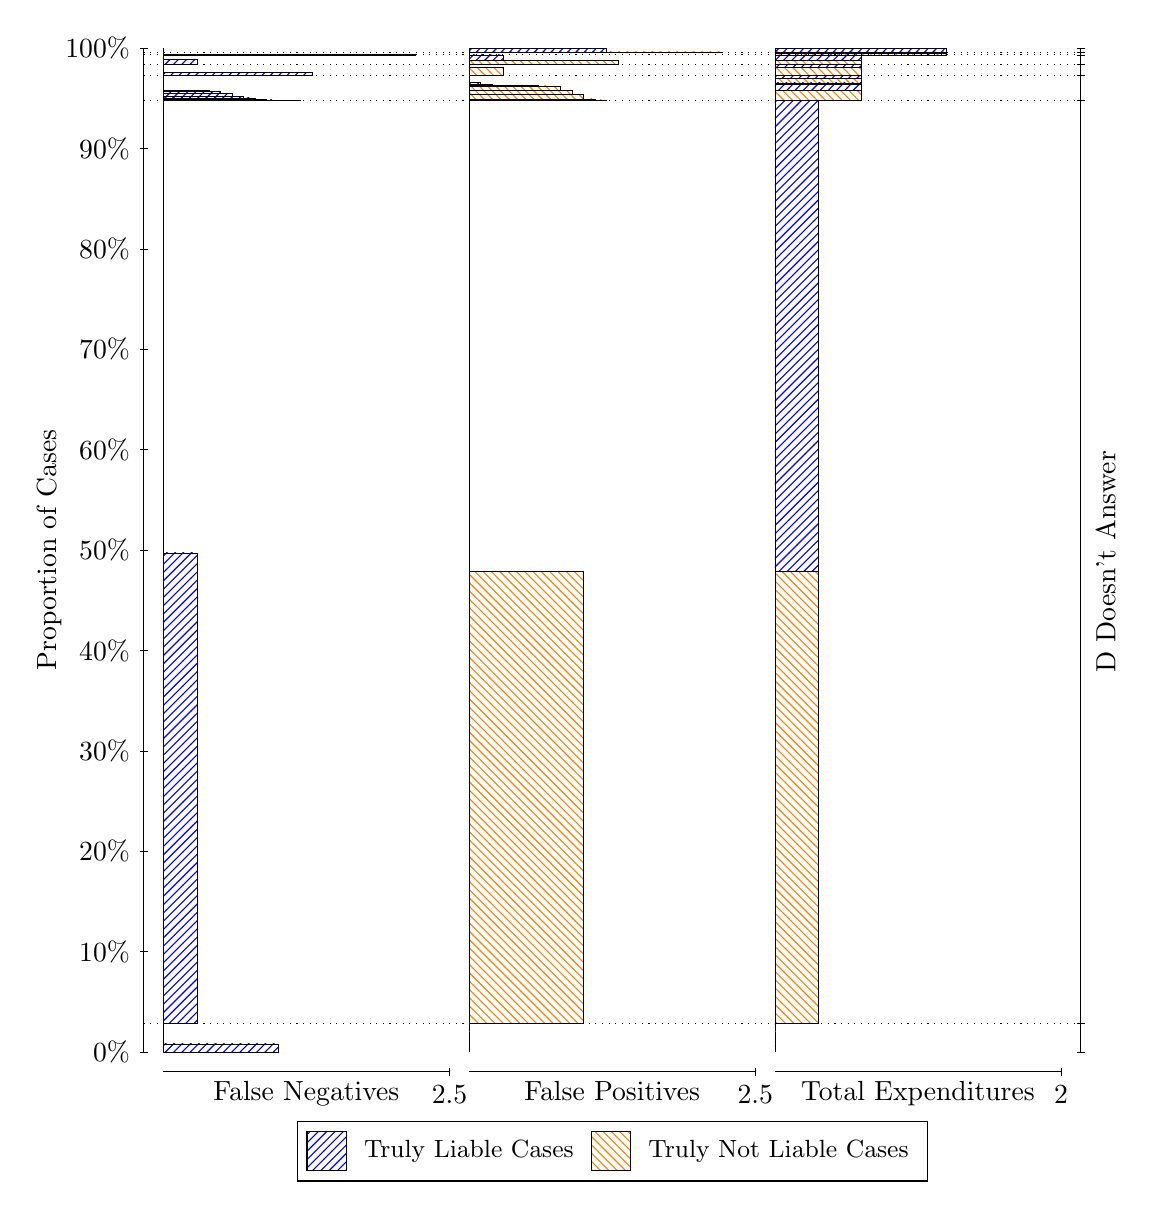
\begin{tikzpicture}
\draw[black, very thin] (1.5,1.75) -- (1.5,14.5);
\node[rotate=90, text=black, anchor=center] at (0.3, 8.125) {Proportion of Cases};
\draw[black, very thin] (1.45,1.75) -- (1.55,1.75);
\node[text=black, anchor=east] at (1.45, 1.75) {0\%};
\draw[black, very thin] (1.45,3.025) -- (1.55,3.025);
\node[text=black, anchor=east] at (1.45, 3.025) {10\%};
\draw[black, very thin] (1.45,4.3) -- (1.55,4.3);
\node[text=black, anchor=east] at (1.45, 4.3) {20\%};
\draw[black, very thin] (1.45,5.575) -- (1.55,5.575);
\node[text=black, anchor=east] at (1.45, 5.575) {30\%};
\draw[black, very thin] (1.45,6.85) -- (1.55,6.85);
\node[text=black, anchor=east] at (1.45, 6.85) {40\%};
\draw[black, very thin] (1.45,8.125) -- (1.55,8.125);
\node[text=black, anchor=east] at (1.45, 8.125) {50\%};
\draw[black, very thin] (1.45,9.4) -- (1.55,9.4);
\node[text=black, anchor=east] at (1.45, 9.4) {60\%};
\draw[black, very thin] (1.45,10.675) -- (1.55,10.675);
\node[text=black, anchor=east] at (1.45, 10.675) {70\%};
\draw[black, very thin] (1.45,11.95) -- (1.55,11.95);
\node[text=black, anchor=east] at (1.45, 11.95) {80\%};
\draw[black, very thin] (1.45,13.225) -- (1.55,13.225);
\node[text=black, anchor=east] at (1.45, 13.225) {90\%};
\draw[black, very thin] (1.45,14.5) -- (1.55,14.5);
\node[text=black, anchor=east] at (1.45, 14.5) {100\%};

\draw[black, very thin] (13.4,1.75) -- (13.4,14.5);
\draw[black, very thin] (13.35,1.75) -- (13.45,1.75);
\node[anchor=west] at (13.35, 1.75) {};
\draw[black, very thin] (13.35,2.1119) -- (13.45,2.1119);
\node[anchor=west] at (13.35, 2.1119) {};
\draw[black, very thin] (13.35,13.834) -- (13.45,13.834);
\node[anchor=west] at (13.35, 13.834) {};
\draw[black, very thin] (13.35,14.154) -- (13.45,14.154);
\node[anchor=west] at (13.35, 14.154) {};
\draw[black, very thin] (13.35,14.29) -- (13.45,14.29);
\node[anchor=west] at (13.35, 14.29) {};
\draw[black, very thin] (13.35,14.414) -- (13.45,14.414);
\node[anchor=west] at (13.35, 14.414) {};
\draw[black, very thin] (13.35,14.443) -- (13.45,14.443);
\node[anchor=west] at (13.35, 14.443) {};
\draw[black, very thin] (13.35,14.5) -- (13.45,14.5);
\node[anchor=west] at (13.35, 14.5) {};

\draw[black, very thin, pattern color=blue, pattern=north east lines] (1.75,1.75) rectangle (3.2033,1.8523);
\draw[black, very thin, pattern color=orange, pattern=north west lines] (1.75,1.8523) rectangle (1.75,2.1119);
\draw[black, very thin, pattern color=blue, pattern=north east lines] (1.75,2.1119) rectangle (2.186,8.0895);
\draw[black, very thin, pattern color=orange, pattern=north west lines] (1.75,8.0895) rectangle (1.75,13.834);
\draw[black, very thin, pattern color=blue, pattern=north east lines] (1.75,13.834) rectangle (3.494,13.836);
\draw[black, very thin, pattern color=blue, pattern=north east lines] (1.75,13.836) rectangle (3.3487,13.838);
\draw[black, very thin, pattern color=blue, pattern=north east lines] (1.75,13.838) rectangle (3.2033,13.841);
\draw[black, very thin, pattern color=blue, pattern=north east lines] (1.75,13.841) rectangle (3.058,13.844);
\draw[black, very thin, pattern color=blue, pattern=north east lines] (1.75,13.844) rectangle (3.058,13.845);
\draw[black, very thin, pattern color=blue, pattern=north east lines] (1.75,13.845) rectangle (2.9127,13.867);
\draw[black, very thin, pattern color=blue, pattern=north east lines] (1.75,13.867) rectangle (2.7673,13.889);
\draw[black, very thin, pattern color=blue, pattern=north east lines] (1.75,13.889) rectangle (2.622,13.928);
\draw[black, very thin, pattern color=blue, pattern=north east lines] (1.75,13.928) rectangle (2.4767,13.948);
\draw[black, very thin, pattern color=blue, pattern=north east lines] (1.75,13.948) rectangle (2.3313,13.962);
\draw[black, very thin, pattern color=orange, pattern=north west lines] (1.75,13.962) rectangle (1.75,14.154);
\draw[black, very thin, pattern color=blue, pattern=north east lines] (1.75,14.154) rectangle (3.6393,14.195);
\draw[black, very thin, pattern color=orange, pattern=north west lines] (1.75,14.195) rectangle (1.75,14.29);
\draw[black, very thin, pattern color=blue, pattern=north east lines] (1.75,14.29) rectangle (2.186,14.359);
\draw[black, very thin, pattern color=orange, pattern=north west lines] (1.75,14.359) rectangle (1.75,14.414);
\draw[black, very thin, pattern color=blue, pattern=north east lines] (1.75,14.414) rectangle (4.9473,14.423);
\draw[black, very thin, pattern color=orange, pattern=north west lines] (1.75,14.423) rectangle (1.75,14.443);
\draw[black, very thin, pattern color=orange, pattern=north west lines] (1.75,14.443) rectangle (1.75,14.452);
\draw[black, very thin, pattern color=blue, pattern=north east lines] (1.75,14.452) rectangle (1.75,14.5);
\draw[black, very thin, pattern color=orange, pattern=north west lines] (5.6333,1.75) rectangle (5.6333,2.0095);
\draw[black, very thin, pattern color=blue, pattern=north east lines] (5.6333,2.0095) rectangle (5.6333,2.1119);
\draw[black, very thin, pattern color=orange, pattern=north west lines] (5.6333,2.1119) rectangle (7.0867,7.856);
\draw[black, very thin, pattern color=blue, pattern=north east lines] (5.6333,7.856) rectangle (5.6333,13.834);
\draw[black, very thin, pattern color=orange, pattern=north west lines] (5.6333,13.834) rectangle (7.3773,13.842);
\draw[black, very thin, pattern color=orange, pattern=north west lines] (5.6333,13.842) rectangle (7.232,13.855);
\draw[black, very thin, pattern color=orange, pattern=north west lines] (5.6333,13.855) rectangle (7.0867,13.915);
\draw[black, very thin, pattern color=orange, pattern=north west lines] (5.6333,13.915) rectangle (6.9413,13.964);
\draw[black, very thin, pattern color=orange, pattern=north west lines] (5.6333,13.964) rectangle (6.796,14.014);
\draw[black, very thin, pattern color=orange, pattern=north west lines] (5.6333,14.014) rectangle (6.6507,14.018);
\draw[black, very thin, pattern color=orange, pattern=north west lines] (5.6333,14.018) rectangle (6.5053,14.021);
\draw[black, very thin, pattern color=orange, pattern=north west lines] (5.6333,14.021) rectangle (6.36,14.023);
\draw[black, very thin, pattern color=orange, pattern=north west lines] (5.6333,14.023) rectangle (6.2147,14.025);
\draw[black, very thin, pattern color=blue, pattern=north east lines] (5.6333,14.025) rectangle (5.924,14.04);
\draw[black, very thin, pattern color=blue, pattern=north east lines] (5.6333,14.04) rectangle (5.7787,14.059);
\draw[black, very thin, pattern color=blue, pattern=north east lines] (5.6333,14.059) rectangle (5.6333,14.154);
\draw[black, very thin, pattern color=orange, pattern=north west lines] (5.6333,14.154) rectangle (6.0693,14.25);
\draw[black, very thin, pattern color=blue, pattern=north east lines] (5.6333,14.25) rectangle (5.6333,14.29);
\draw[black, very thin, pattern color=orange, pattern=north west lines] (5.6333,14.29) rectangle (7.5227,14.346);
\draw[black, very thin, pattern color=blue, pattern=north east lines] (5.6333,14.346) rectangle (6.0693,14.414);
\draw[black, very thin, pattern color=orange, pattern=north west lines] (5.6333,14.414) rectangle (5.6333,14.434);
\draw[black, very thin, pattern color=blue, pattern=north east lines] (5.6333,14.434) rectangle (5.6333,14.443);
\draw[black, very thin, pattern color=orange, pattern=north west lines] (5.6333,14.443) rectangle (8.8307,14.452);
\draw[black, very thin, pattern color=blue, pattern=north east lines] (5.6333,14.452) rectangle (7.3773,14.5);
\draw[black, very thin, pattern color=orange, pattern=north west lines] (9.5167,1.75) rectangle (9.5167,2.0095);
\draw[black, very thin, pattern color=blue, pattern=north east lines] (9.5167,2.0095) rectangle (9.5167,2.1119);
\draw[black, very thin, pattern color=orange, pattern=north west lines] (9.5167,2.1119) rectangle (10.062,7.856);
\draw[black, very thin, pattern color=blue, pattern=north east lines] (9.5167,7.856) rectangle (10.062,13.834);
\draw[black, very thin, pattern color=orange, pattern=north west lines] (9.5167,13.834) rectangle (10.607,13.958);
\draw[black, very thin, pattern color=blue, pattern=north east lines] (9.5167,13.958) rectangle (10.607,14.039);
\draw[black, very thin, pattern color=orange, pattern=north west lines] (9.5167,14.039) rectangle (10.607,14.048);
\draw[black, very thin, pattern color=blue, pattern=north east lines] (9.5167,14.048) rectangle (10.607,14.058);
\draw[black, very thin, pattern color=orange, pattern=north west lines] (9.5167,14.058) rectangle (10.607,14.117);
\draw[black, very thin, pattern color=blue, pattern=north east lines] (9.5167,14.117) rectangle (10.607,14.154);
\draw[black, very thin, pattern color=orange, pattern=north west lines] (9.5167,14.154) rectangle (10.607,14.25);
\draw[black, very thin, pattern color=blue, pattern=north east lines] (9.5167,14.25) rectangle (10.607,14.29);
\draw[black, very thin, pattern color=orange, pattern=north west lines] (9.5167,14.29) rectangle (10.607,14.346);
\draw[black, very thin, pattern color=blue, pattern=north east lines] (9.5167,14.346) rectangle (10.607,14.414);
\draw[black, very thin, pattern color=orange, pattern=north west lines] (9.5167,14.414) rectangle (11.697,14.434);
\draw[black, very thin, pattern color=blue, pattern=north east lines] (9.5167,14.434) rectangle (11.697,14.443);
\draw[black, very thin, pattern color=orange, pattern=north west lines] (9.5167,14.443) rectangle (11.697,14.452);
\draw[black, very thin, pattern color=blue, pattern=north east lines] (9.5167,14.452) rectangle (11.697,14.5);
\draw[black, dotted] (1.5,2.1119) -- (13.4,2.1119);
\draw[black, dotted] (1.5,13.834) -- (13.4,13.834);
\draw[black, dotted] (1.5,14.154) -- (13.4,14.154);
\draw[black, dotted] (1.5,14.29) -- (13.4,14.29);
\draw[black, dotted] (1.5,14.414) -- (13.4,14.414);
\draw[black, dotted] (1.5,14.443) -- (13.4,14.443);
\draw[black, very thin] (1.75,1.5) -- (5.3833,1.5);
\node[text=black, anchor=north] at (3.5667, 1.5) {False Negatives};
\draw[black, very thin] (5.3833,1.45) -- (5.3833,1.55);
\node[text=black, anchor=north] at (5.3833, 1.45) {2.5};

\draw[black, very thin] (5.6333,1.5) -- (9.2667,1.5);
\node[text=black, anchor=north] at (7.45, 1.5) {False Positives};
\draw[black, very thin] (9.2667,1.45) -- (9.2667,1.55);
\node[text=black, anchor=north] at (9.2667, 1.45) {2.5};

\draw[black, very thin] (9.5167,1.5) -- (13.15,1.5);
\node[text=black, anchor=north] at (11.333, 1.5) {Total Expenditures};
\draw[black, very thin] (13.15,1.45) -- (13.15,1.55);
\node[text=black, anchor=north] at (13.15, 1.45) {2};


\node[text=black, centered, rotate=90] at (13.72, 7.9727) {D Doesn't Answer};






\draw (7.449999999999999,1.5) node[draw=none] (baseCoordinate) {};
\begin{scope}[align=center]
        \matrix[scale=0.5, draw=black, below=0.5cm of baseCoordinate, nodes={draw}, column sep=0.1cm]{
            \node[rectangle, draw, minimum width=0.5cm, minimum height=0.5cm, pattern color=blue, pattern=north east lines] {}; &
            \node[draw=none, font=\small, text=black] (B) {Truly Liable Cases}; &
            \node[rectangle, draw, minimum width=0.5cm, minimum height=0.5cm, pattern color=orange, pattern=north west lines] {}; &
            \node[draw=none, font=\small, text=black] (B) {Truly Not Liable Cases}; \\
            };
\end{scope}

\end{tikzpicture}
\end{document}